% Workbench figure (appendix). Screenshots of the synthetic demo examples/materials-testing-lab/atoms.yaml
% with the offline rules provider (mock), retaken on 14 Nov 2026 at commit 5ffd56e (the tool the paper describes;
% frontend built from that commit); numbers in paper/inputs/demo-materials-testing-lab-5ffd56e-2026-11-14.json, equal to
% those of the first take at 0d7aadc (paper/inputs/demo-materials-testing-lab-2026-11-14.json). No benchmark content.
\begin{figure}[!htbp]
  \centering
  \begin{minipage}[t]{0.485\textwidth}
    \vspace{0pt}
    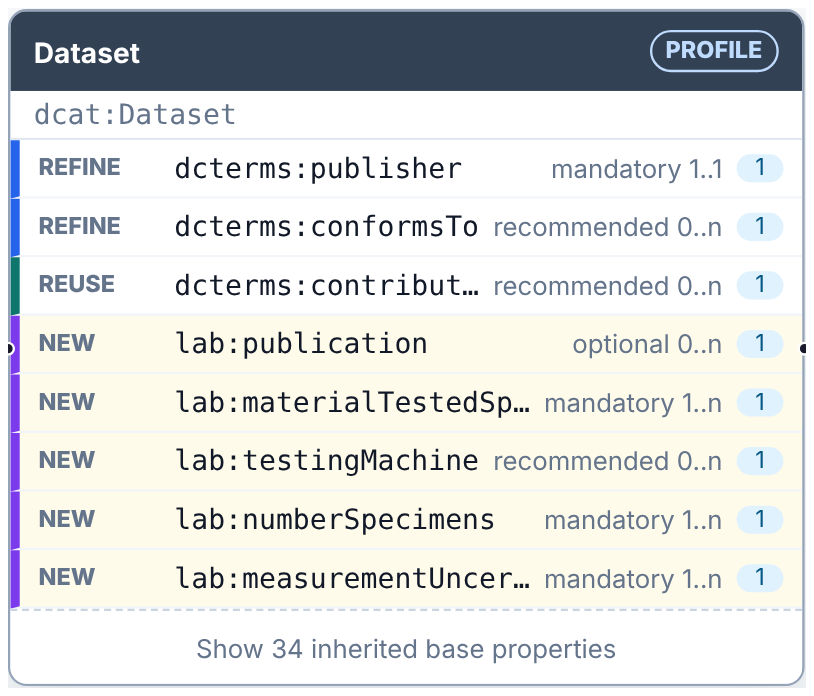
\includegraphics[width=\linewidth]{figures/wb-canvas-dataset.png}\\[0.6ex]
    {\scriptsize (a) Canvas card of \term{dcat:Dataset}}\\[1.2ex]
    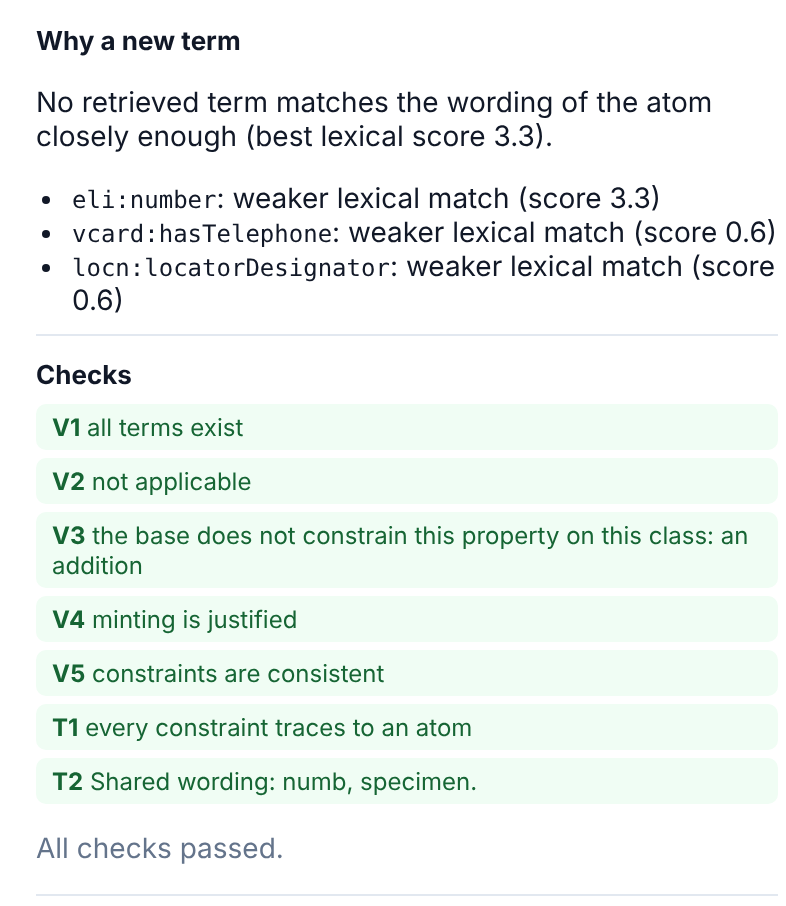
\includegraphics[width=\linewidth]{figures/wb-inspector-mint-bottom.png}\\[0.6ex]
    {\scriptsize (c) Inspector, continued: rejected candidates and checks}
  \end{minipage}\hfill
  \begin{minipage}[t]{0.485\textwidth}
    \vspace{0pt}
    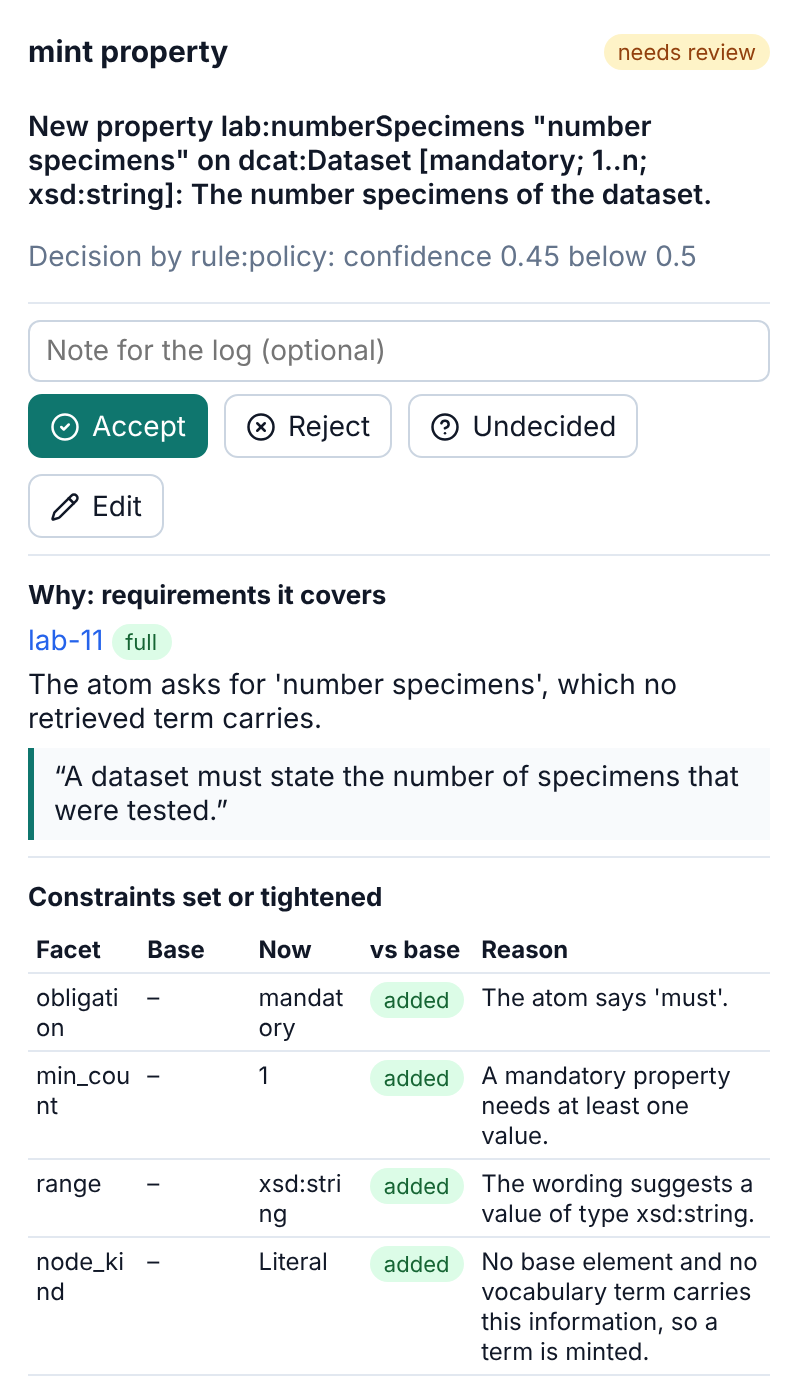
\includegraphics[width=\linewidth]{figures/wb-inspector-mint-top.png}\\[0.6ex]
    {\scriptsize (b) Inspector of one minted property}
  \end{minipage}
  \caption{The workbench on the synthetic demo of Table~\ref{tab:criteria}, run with the offline rules provider
    instead of a model, so the choices shown are a lexical baseline's (\term{xsd:string} for a count).
    (a)~Rows that tighten a base constraint (REFINE), add an existing term (REUSE) or mint one (NEW),
    with obligation, cardinality and atoms covered; shaded rows wait for review. (b)~The decision and why the
    machine left it open, the covered atom with its verbatim quote, and one justification per constraint, with
    base and new value. (c)~The candidates the mint rejected, with their lexical scores, and the checks.}
  \label{fig:workbench}
\end{figure}
